\section*{Analysis}
\label{Analyse}
%
Based on the results presented in the previous section it is possible to analyze how well a fit the BTL-model is. 
\\\\
The number of SST violations is 25 and that is a bit higher than desired. Because the SST violations is a bit high it is unlikely that any model will fit, but because the number of WST violations is only two, this could give the possibility of rank ordering. 
\\\\
The results from the Chi-square test shows a p-value at 0.3725. This value is above the significant level at 0.1 at therefore the test results show that there is no significant difference and the BTL-model is accepted. 

\noindent To understand what the analysis shows, the scale values and confidence intervals is plotted and shown in \autoref{fig:Confidens}. 

\begin{figure}[H]
\centering
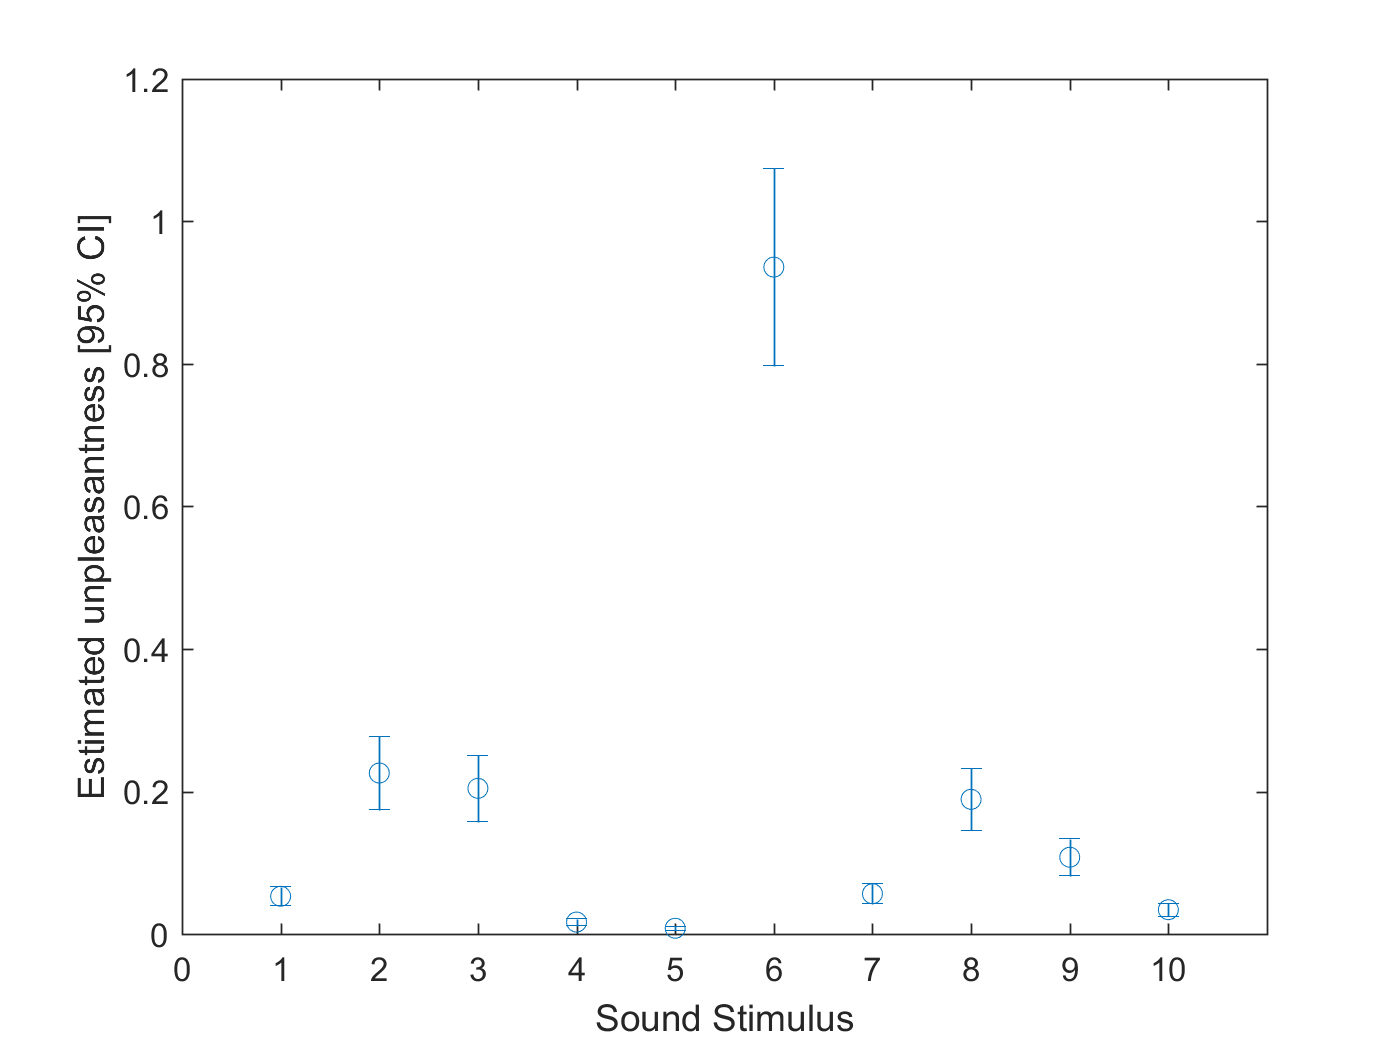
\includegraphics[width = 0.90\textwidth]{Figure/Confidens.png} 
\caption{Scale values and 95 \% confidence intervals}
\label{fig:Confidens}
\end{figure}

\noindent From the plot at \autoref{fig:Confidens} it is clear that the scale value for sound number six is significant different from all the other values. The rest of the scale values is split into to groups. The group with the highest values consists of sound number two, three, eight and nine. The scale values for these sound is not significant different from each other but they are all significant different from the values of the sounds in the last group, that consist of sound number one, four, five, seven and ten. 

%First check for stochastic transitivity violations, WST, MST, SST. (there is no Matlab function for this, so you’ll have to do some programming yourself)
%How good a fit does your solution have? (interpret the result of the chi-square test).
%What does your analysis show? (Plot your scale values and 95\% confidence intervals).


